\section{Исследование моделей}
\label{sec:Chapter4} \index{Chapter4}

В данной главе я опишу поставленный эксперимент по исследованию моделей и приведу полученные результаты.

\subsection{Описание эксперимента}

Эксперимент, как и вся работа разделен на две части: исследование моделей распознавания ключевых точек на теле человека и исследование моделей классификации поз человека.

В первой части работы были выбраны несколько моделей распознавания ключевых точек на теле человека и проведен их анализ. Для выбора моделей использовались некоторые критерии:

\begin{itemize}
	\item Доступность модели для исследований\\
	Необходимо оценить длительность установки и возможности работы с различными операционными системами. Эксперимент проводился на платформе Google Colab, поэтому необходимо было рассмотреть возможность использования модели на в Colaboratory.
	\item Новизна модели\\
	Представленная выборка была создана в основном в 2010-х, но модель DeepPose является самой старой. Новые разработки опирались на результаты, полученные в ней, и таким образом получали более хорошие результаты.
	\item Наличие документации\\
	Все модели производят классификацию по двум осям изображения: высота и ширина, а также по параметру видимость ключевой точки. Некоторые модели выдают данные нормированные на размер изображения (число из отрезка [0,1]), а некоторые точное значение в пикселях. Поэтому для работы необходимо было понимать как работает API модели, какие у нее входные - выходные данные.
	\item Тренировка модели на датасете COCO\\
	Все используемые претренированные модели были обучены на наборе данных COCO \cite{COCO_topology} в совместительстве с каким-либо другим датасетом. В некоторых  примерах не было возможности использовать претренированную модель и из-за этого они были отсеяны.
\end{itemize}

В итоге было выбрано 4 модели наиболее подходящие под критерии:
\begin{enumerate}
	\item BlazePose
	\item MoveNet.SinglePose
	\item OpenPose
	\item MMpose
\end{enumerate}

Для проведения качественного анализа и выявления лучшей модели необходимо их сравнить. Поэтому рассмотрим метрики, которые подходят для задач в 2-х мерном пространстве:

\begin{itemize}
	\item Percentage of Detection Joints\\
	PDJ оценивает точность распознавания ключевой точки в зависимости от диагональных размеров человека. При рассмотрении задачи распознавания человека мы получаем координаты точек, которые характеризуют прямоугольник, внутри которого вписан человек. Диагональ этого прямоугольника используется при высчитывании метрики PDJ (см. рис \autoref{fig:PDJ}). Формулу можно представить в следующем виде:
	\begin{equation}
		PDJ = \frac{\sum_{i=1}^{n} bool(d_i < threshold * diag)}{n},
	\end{equation}
	
	где\\
	$d_i$ - расстояние между предсказанной и правильной точкой,\\
	$threshold$ - порог, задаваемый исследователем,\\
	$diag$ - размер диагонали прямоугольника, внутри которого находится человек,\\
	$bool()$ - логическое условие, возвращает 1, если оно верно и 0 в ином случае,\\
	$n$ - размер выборки.
	
	С помощью значения порога можно варьировать допустимую погрешность расстояния между истинной и предсказанной точками.
	\begin{figure}[h]
	\centering
	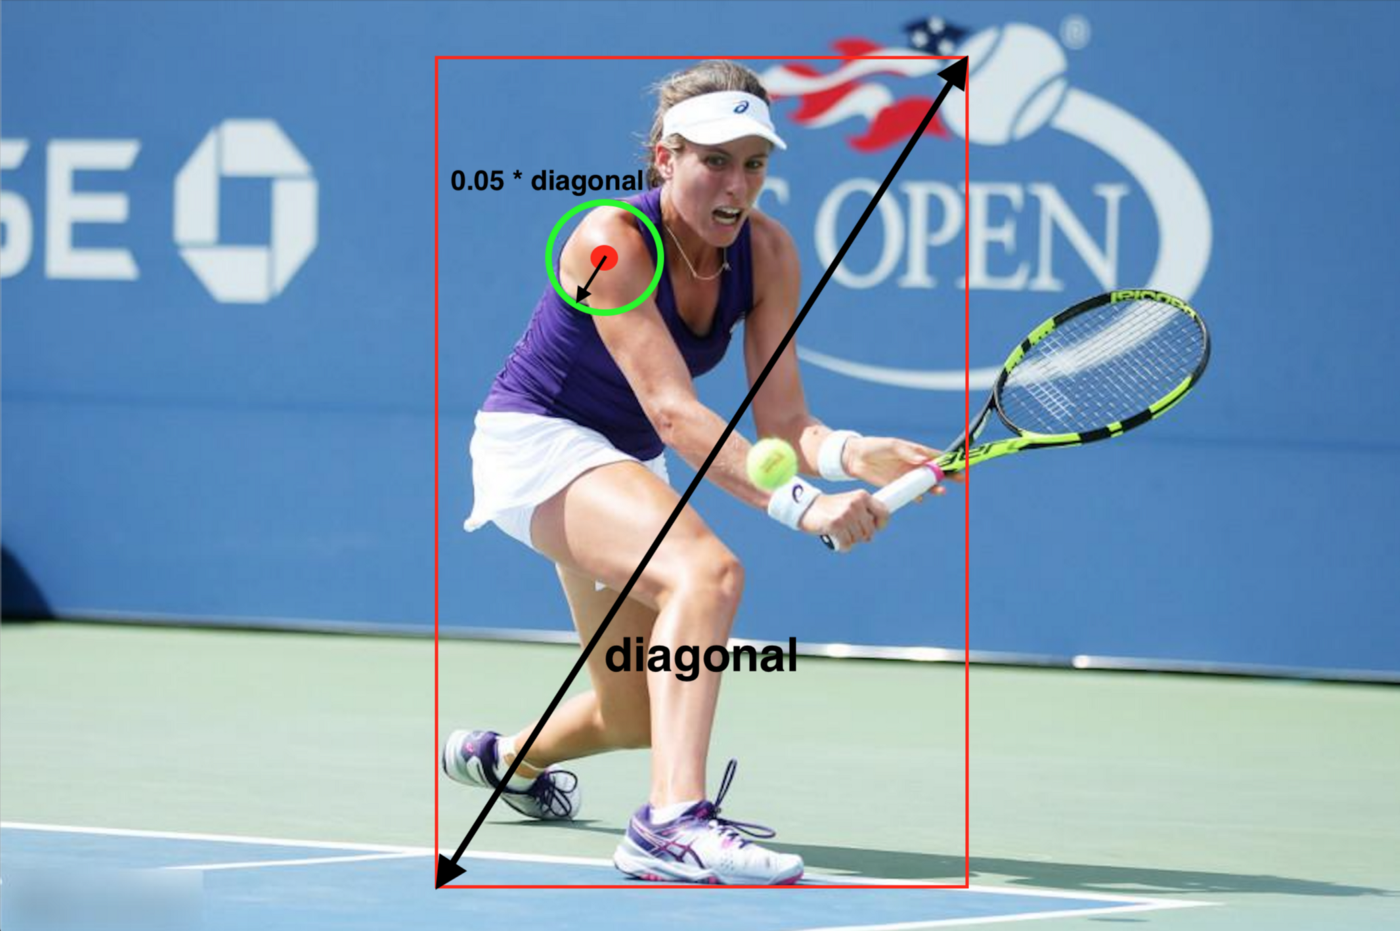
\includegraphics[width=\textwidth * 4 / 5]{./images/PDJ}
	\caption{Визуальное представление метрики PDJ.\\ \href{hhttps://miro.medium.com/max/1400/1*dJhVudwq7pb_xl3yPEH37Q.jpeg}{Оригинальное изображение}}
	\label{fig:PDJ}
\end{figure}

	\item Percentage of Correct Key-points\\
	PCK очень похожа на предыдущую метрику, только погрешность рассматривается относительно высоты человека. Формулу можно представить в следующем виде:
	\begin{equation}
		PDJ = \frac{\sum_{i=1}^{n} bool(d_i < threshold * body_height)}{n},
	\end{equation}
	
	где\\
	$d_i$ - расстояние между предсказанной и правильной точкой,\\
	$threshold$ - порог, задаваемый исследователем,\\
	$body_height$ - высота прямоугольника, внутри которого находится человек,\\
	$bool()$ - логическое условие, возвращает 1, если оно верно и 0 в ином случае,\\
	$n$ - размер выборки.
	
	В представленных выше двух метриках необходимо знать размеры прямоугольника, ограничивающего человека. Для этого необходимо использовать модель распознавания объектов, которая будет давать нам эти данные. При работе с метрикой PCK можно обойтись без такой модели, потому что во всех топологиях есть точки, которые обозначают верхнюю и нижнюю границы человека. Отсюда погрешность вычисления через модель и вычисления разности ординат верхней и нижней точек будет мала. Что требует меньше затрат для оценки.
	
	\item Object Key-point Similarity\\
	OKS является основной при оценке задачи Keypoint Detection COCO \cite{COCO_topology}. Она использует третью координату выходного предсказания и расстояние между реальной и предсказанной точками. Формулу можно представить в следующем виде:
	\begin{equation}
		OKS = \frac{\sum_{i} exp\left( - d_i^2 / 2s^2k_i^2\right)\delta\left(v_i > 0\right)}{\sum_{i} \delta\left(v_i > 0\right)},
	\end{equation}
	где\\
	$d_i$ - расстояние между предсказанной и правильной точкой,\\
	$s$ - площадь объекта,\\
	$k_i$ - константа ключевой точки, контролирующаю спад,\\
	$v_i$ - видимость.
	
	При оценке задачи детекции ключевых точек COCO вводится метрика Average Precision (AP) через OKS. Изменяя границу допустимого значения OKS можно получать различные значения precision и AP.
\end{itemize}

(Если упею, то допишу вторую часть. Если нет, то просто уберу эти слова)

\subsection{Поиск данных}

Первым делом необходимо было проверить модели на неразмеченных данных. Для этого были выбраны фотографии высокого разрешения, где человек изобраен во весь рост. (ФОТОГРАФИИ)

Для качественной оценки работы моделей с помощью метрик необходимо было найти размеченные данные. Приведу описание датасетов, которые были мной рассмотрены:

\begin{itemize}
	\item COCO Dataset и MPII\\
	Данные наборы являются основными при работе с компьютерным зрением и большинство исследователей используют их как тренировочные для своих моделей. Поэтому использовать их в качестве тестовых не целесообразно. \cite{COCO_dataset, MPII_dataset}
	\item HUMAN 3.6M\\
	Данные собирались специально для задачи классификации движений человека в студии. С помощью датчиков фиксировались положения всех суставов и ключевых точек. Это идеальный датасет, но доступ к нему ограничен и создатель не выходит на связь. \cite{h36m_pami}
	\item LSP\\
	Данные собраны со спортивных соревнований и предобработаны до обозначения одного человека на изображении размером не менее 150 пикселей в высоту. Единственная проблема - не описаны точки на лице, поэтому оценивать можно только распознавание суставов или, другими словами, точек на теле человека. \cite{LSP}
\end{itemize}

Выше были представлены наборы данных для задачи распознавания точек на теле человека. Но основной темой является классификация движений человека. Поэтому необходимы фотографии с меткой класса для позы, представленной на данных. Некоторые из уже представленных (COCO, MPII) тоже могут использоваться для классификации позы, но по тем же причинам, что и описаны выше, они не будут рассмотрены в эксперименте. Приведу описание датасетов для классификации движения человека по позе на изображении:

\begin{itemize}
	\item HPC/mmakos (ССЫЛКА)\\
	Убедиться в реальной работоспобобности датасета
	\item Stanford-40 (ССЫЛКА)\\
	\item Yoga-82 (ССЫЛКА)\\
\end{itemize}

Итого были выбраны наборы данных: LSP и ... (ФОТОГРАФИИ ИЗ ДАТАСЕТА)

\subsection{Полученные результаты эксперимента}

Рассмотрим результаты первой части работы.

Для каждой модели была рассмотрена локализация ключевых точек на фотографиях высокого качества (ССЫЛКА НА ФОТО ВЫШЕ), а также набор данных низкого качества с обработанными изображениями.

Метрики были рассчитаны с порогами 0.05, 0.2, 0.5. В дополнение к этому был проведен временной анализ классификации одного изображения в среднем по целому датасету.

Перейдем к результатам по каждой модели.

\begin{large}
BlazePose
\end{large}

ФОТОГРАФИИ МОИ И РЕЗУЛЬТАТЫ В ТАБЛИЦЕ

\begin{large}
MoveNet.SinglePose
\end{large}

ФОТОГРАФИИ МОИ И РЕЗУЛЬТАТЫ В ТАБЛИЦЕ

\begin{large}
OpenPose
\end{large}

ФОТОГРАФИИ МОИ И РЕЗУЛЬТАТЫ В ТАБЛИЦЕ

\begin{large}
MMPose
\end{large}

ФОТОГРАФИИ МОИ И РЕЗУЛЬТАТЫ В ТАБЛИЦЕ

Вторую часть работы пишем...

\newpage